\section{Scrolling in Week Schedule}
\userstory{As a user, I would like to be able to have long schedules which are scroll-able, such that I can schedule more in a single day.}

\begin{wrapfigure}{r}{0.45\textwidth} 
    \centering
        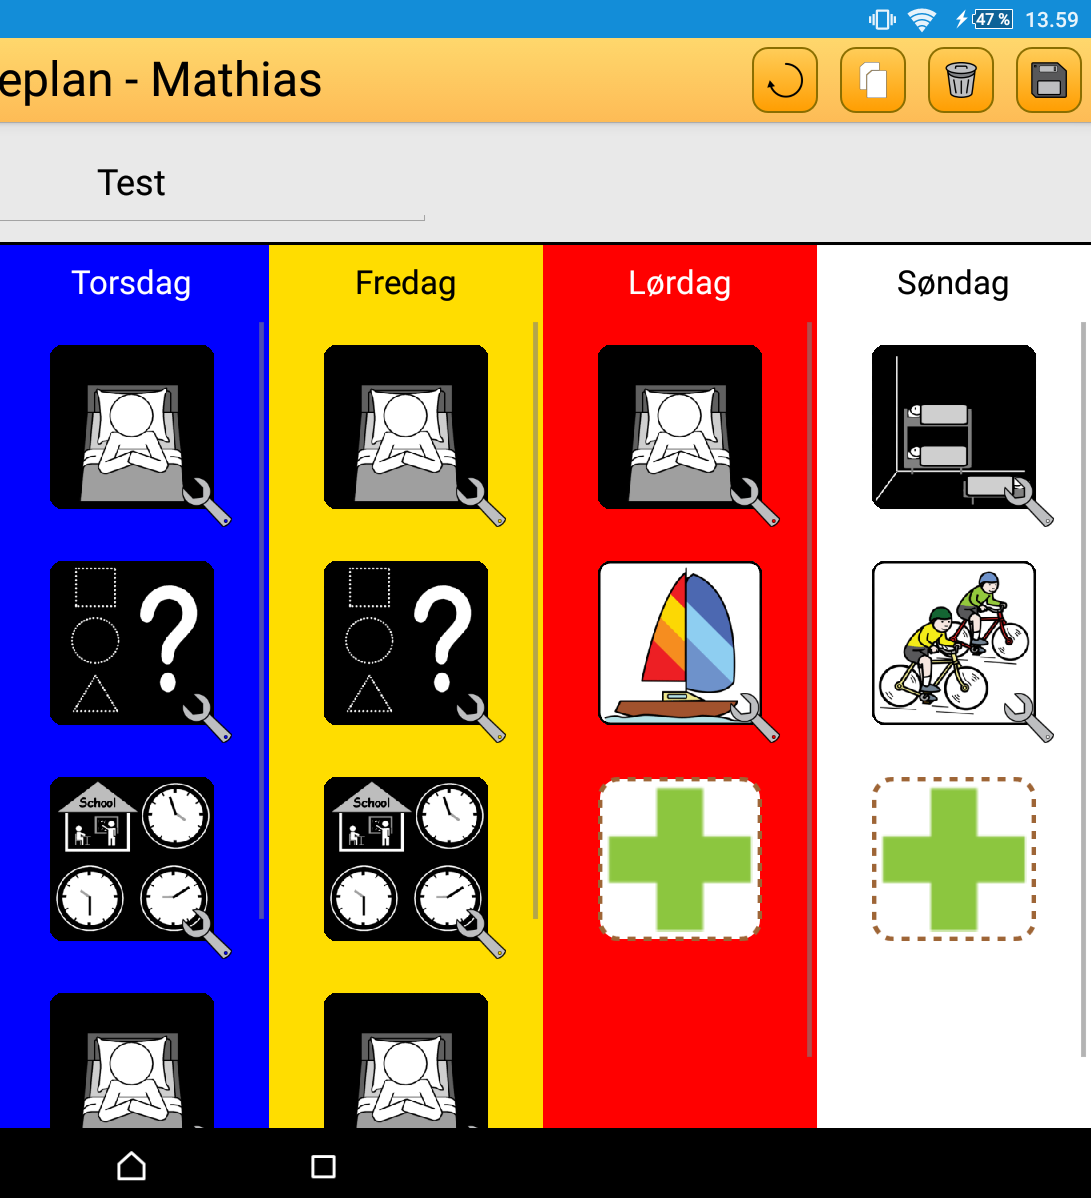
\includegraphics[width=0.4\textwidth]{figures/img/screenshots/weekplan_schedule.png}
    \caption{An example of a week schedule.}
    \label{fig:weekschedule}
    \vspace{-20pt}
\end{wrapfigure}

This section presents the resolution of the aforementioned user story, which was given a \phigh--priority by the PO.

First we will explain the reason for this user story, then two solutions will be presented and finally the solution we choose to implement is presented. 

\myref{fig:weekschedule} shows a cutout from a week schedule. 
Before the changes presented in this section it was not possible to scroll while touching a pictogram. 
It was implemented such that if you were logged in as a guardian and dragged while touching a pictogram you would change the order of the pictograms rather than scrolling through the view.
In order to scroll you would have to touch the background in each daily schedule or by touching the scrollbar as seen on \myref{fig:weekschedule}.

This resulted in scrolling being difficult since it was hard to avoid accidentally tapping a pictogram, and needed to be changed.
In order to increase the number of possible scrolling areas it was decided to make it possible to scroll while touching a pictogram. \kim{What do you mean by number of scrolling areas? please elaborate.}
Because of this choice a new way to change the position of pictograms in the week schedule is also needed, since if dragging on a pictogram is supposed to scroll,\kim{please rephrase.} the current implementation of reordering pictograms must be removed. 
\kim{to improve this section then add some reason for why scrolling should be supported by dragging. }
\bigskip \noindent
At the sprint planning meeting the following tasks were made for this user story:
\begin{enumberate}
	\item \subtask{Make the entire day's view scrollable}
	\item \subtask{Redesign the reordering mode}
\end{enumberate}
\kim{This listing of tasks seems like a new thing. Are you going to add these to all user stories?}
\kim{I think that introduction is require before you can start a new subsection. Like ``In the next section we discuss ...''}
\subsection*{To Button or Not to Button} % That is the question
Currently the GIRAF application suite has buttons in the top of the screen which are used for actions such as entering modes for deleting or copying and for saving etc. 
One possible solution for dragging is to create yet another button to change the current mode of the week schedule application such that dragging on a pictogram results in dragging a pictogram instead of scrolling.
However, this solution would still be problematic for when you enter the dragging mode and then want to scroll to the pictogram you want to drag.
Another solution is inspired by how many other applications including the standard Android OS and iOS implement dragging of icons.
Longpressing\footnote{An extended tap for a given period set by the OS} a button or an icon in order to start dragging an icon is used in both Android OS and iOS mainly on the home screen to move change the position of different apps.
The same technique can be used in the week schedule, a longpress on a pictogram will cause the application to now drag the pictogram along the movement of the user.
This solution is preferable to the other as users might already associate a longpress with this functionality and therefore we would adhere to the design guideline of recognisable design \cite[p.~51]{DESIGNBOOK}.
As such we deem this the better solution, the next subsection will introduce how this is implemented in the application.
\kim{You just argued that going into a edit mode was bad because you would not be able to scroll while in this mode. As I understand your design then you still have this problem.}

\subsection*{The Implementation}
\kim{This is the first time that the implementation have started with a ``The implementation'' section headline. Please make it consistent with the rest of the sections..}
The implementation is separated into two parts, each corresponding to one of the tasks mentioned above. 
\subsubsection*{\subtask{Make the entire day's view scrollable}} \kim{Why is this headline in quotes?}
To resolve this task, firstly we disable the previous way to drag pictograms and the make the entire view scrollable. 
Previously a boolean variable called \texttt{isDraggable}, for each pictogram in the week schedule, was set to true. 
Changing this to false disabled the ability to reorder pictograms by dragging them. 
However this did not enable scrolling by dragging on top of a pictogram. \kim{This sentence make it sound like that you were surprised by this fact, rephrase it such that it is a fact that you state.}

The touch information is sent to the touch handler, \texttt{onTouch(MotionEvent)}, for the pictogram, and not the weekday view itself when attempting to drag on-top of a pictogram. 
Therefore each child view (i.e. a pictogram) has to send the information of the motion to its parent view (i.e. a weekday). 
The information in question is an amount of pixels for the parent view to scroll. 
The code calculating this is shown in \myref{lst:actionmove}, and is part of the \texttt{onTouch(MotionEvent)} method, which handles touch input. 
Line 1 decides if a scroll should happen or not, it should happen if the user dragged more than two pixels. 
In line 3 the distance to scroll is calculated, and in line 5-6 this information is sent to the parent, which in this case is weekday.  \kim{This is a good description of the code, more code and more descriptions, please.}

\begin{lstlisting}[floatplacement=h, caption={The code executed when someone performs a move action.}, label={lst:actionmove}] 
if(lastYCoord != -1 && Math.abs(event.getRawY() - lastYCoord) > 2 && !draggable) {
    handler.removeCallbacksAndMessages(null);
    int scrollDistance = (int) (lastYCoord - event.getRawY());
    lastYCoord = event.getRawY();
    ((ScrollView)this.getParent()).scrollTo(0,((ScrollView)this.getParent())
    		.getScrollY() + scrollDistance);
	scrollTime = new Date();

	return true;
}
\end{lstlisting}

\subsubsection*{\subtask{Redesign the reordering mode}}

Next a presentation of how the longpress is implemented.
\myref{lst:longpress} shows the code executed upon long pressing.
It is a function made inside a runnable which means it will be run in its own thread and therefore makes it possible to queue it for execution. \kim{Why would you want to query tasks for going into edit mode? Please explain.}
Lines 3-4 makes it so pictograms can be dragged on the screen and lines 5-7 will if a pictogram is being touched lift it up indicating that the pictogram can be dragged, and the tablet will also vibrate briefly so the user knows they can now drag the pictogram.

\begin{lstlisting}[floatplacement=h, caption={The longpress function which is queued upon a \texttt{MotionEvent\_Down}, i.e. a touch.}, label={lst:longpress}] 
private Runnable mLongPressed = new Runnable() {
    public void run() {
        adapter.setDraggability(true);
        setDraggable(true);
        if(draggingView != null){
            ((PictogramView) draggingView).liftUp();
            vibrator.vibrate(100);
        }
    }
};
\end{lstlisting}
This function is queued when the initial press begins, and if it lasts for more than 500 milliseconds, then it is executed. 
If the press is shorter then it is canceled as shown on line 2 in \myref{lst:actionmove}. 

\bigskip \noindent
In conclusion these fairly small changes result in what we believe to be a more intuitive way to navigate the Week Schedule app based on the assumption that the user is familiar with Android OS and iOS standards; hopefully the customers agree that it is a better solution, which will be disclosed at the customer meeting following sprint 2 end.